%%% start preambling . . .  %%%
\documentclass{article}
% required 

% EMW recommends parskip now instead of \\ too much: https://www.overleaf.com/learn/latex/Articles/How_to_change_paragraph_spacing_in_LaTeX#The_parskip_package ... add \usepackage{parskip} to preamble, delete \\ and see how it looks
\usepackage{parskip}
\usepackage{amsmath}
\usepackage[semicolon]{natbib}
\bibliographystyle{plainnat} %{unsrtnat}
\usepackage{xr-hyper}
\usepackage{hyperref}
\externaldocument[supplement-]{supplement}
\usepackage{booktabs,siunitx}
\usepackage{Sweave}
\usepackage{graphicx}
\usepackage{lipsum}                     % Dummytext % https://tex.stackexchange.com/questions/9796/how-to-add-todo-notes
\usepackage{xargs}                      % Use more than one optional parameter in a new commands
\usepackage[pdftex,dvipsnames]{xcolor}  % Coloured text etc.
\usepackage[colorinlistoftodos,prependcaption,textsize=tiny]{todonotes}
\newcommandx{\unsure}[2][1=]{\todo[linecolor=red,backgroundcolor=red!25,bordercolor=red,#1]{#2}}
\newcommandx{\change}[2][1=]{\todo[linecolor=blue,backgroundcolor=blue!25,bordercolor=blue,#1]{#2}}
\newcommandx{\info}[2][1=]{\todo[linecolor=OliveGreen,backgroundcolor=OliveGreen!25,bordercolor=OliveGreen,#1]{#2}}
\newcommandx{\improvement}[2][1=]{\todo[linecolor=Plum,backgroundcolor=Plum!25,bordercolor=Plum,#1]{#2}}
\newcommandx{\thiswillnotshow}[2][1=]{\todo[disable,#1]{#2}}
% https://tex.stackexchange.com/questions/60209/how-to-add-an-extra-level-of-sections-with-headings-below-subsubsection
\usepackage{titlesec}
\setcounter{secnumdepth}{4}

\titleformat{\paragraph}
{\normalfont\normalsize\bfseries}{\theparagraph}{1em}{}
\titlespacing*{\paragraph}
{0pt}{3.25ex plus 1ex minus .2ex}{1.5ex plus .2ex}

% recommended! Uncomment the below line and change the path for your computer!
 
%put your figures in one place! Also, note that here 'figures' is the folder and 'demoFig' is what each 
% figure produced will be titled plus its number or label (e.g., demoFig-nqpbetter.pdf')
% make your captioning look better
\usepackage[small]{caption}
\setlength{\captionmargin}{30pt}
\setlength{\abovecaptionskip}{0pt}
\setlength{\belowcaptionskip}{10pt}
% optional: muck with spacing
\topmargin -1.5cm        
\oddsidemargin 0.5cm   
\evensidemargin 0.5cm  % same as oddsidemargin but for left-hand pages
\textwidth 15.59cm
\textheight 21.94cm 
% \renewcommand{\baselinestretch}{1.5} % 1.5 lines between lines
\parindent 0pt		  % sets leading space for paragraphs
% optional: cute, fancy headers
\usepackage{fancyhdr}
\pagestyle{fancy}
\fancyhead[LO]{July 2023}
\fancyhead[RO]{Manuscript}
% more optionals! %
% \usepackage[hyphens]{url} % this wraps my URL versus letting it spill across the page, a bad habit LaTeX has
%%% end preambling. %%%

\begin{document}
\Sconcordance{concordance:supplement.tex:supplement.Rnw:%
1 65 1}
 % For RStudio hiccups
\title{{\huge Changes and trends in budburst and leaf flush across Europe and North America} \\A meta-analysis of local adaptation in spring phenology studies}
\author{Ziyun Zeng \& E. M. Wolkovich}
\date{2023}
\maketitle 


\newpage
% Journal ideas: Global Change Biology; Functional Ecology or Journal of Ecology next seem good ... maybe a biogeography journal (though I am not sure if we can afford one) ... maybe New Phytologist but I think they could be picky. 


% Just jotting down and putting some bits you have for abstract for now. 
\begin{abstract}
Climate change forecasting .... plasticity.... adaptation. Spring tree phenology is critical to forecasting ... Despite a long history of study, however, the balance of local adaptation versus plasticity in determining environmental responses is not well understood, especially for spring events. We conducted the first cross-continental meta-analysis of published studies from the peer-reviewed literature that reported spring event dates for a mix of angiosperm and gymnosperm tree species in the northern hemisphere, capturing data from 384 North American provenances and 101 European provenances with observations from 1962 to 2019.  We found ... This is important because... 
\end{abstract}

\section{Introduction}
%emw: FYI this is a first draft -- meaning it still has lots of words, sentences and other bits to fix; but best to do that as we go. 
%emw: I noticed a lot of papers on local adaptation don't always use the term 'local adaptation' so we may want to avoid using it too much? I suspect it may be contested. I also wonder if my advice about definitions was wrong ... but let's definitely save that text for now. 
%emw: We need to 'funnel' in our intros -- until we submit to a plant journal focusing on plants too early is getting too narrow too fast. 

% To optimize ecosystem services for habitat conservation and understand how plants cope with environmental variations, predicting the biological impacts of climate change is of critical importance \citep{botero15}. One of the most important parts of accurate prediction is understanding the relative importance of local adaptation versus plasticity \citep{chevin10}. 
Predicting the biological impacts of climate change has made understanding how organisms cope with environmental variation more urgent \citep{botero15}. In particular, the relative importance of plasticity versus genetic adaptation is vital for prediction \citep{chevin10}, with plasticity expected to allow species to shift more rapidly with climate change than environmental responses based on local adaptation \citep{chevin102, snell18}.

% Local adaptation---how well the growth and adaptive characteristics align with the local climate conditions---influences their ability to thrive and reproduce  \citep{casmey22, kawecki04, anderson12, kim13}. When the selection intensity exceeds gene flow in species that spread over diverse areas, clinal variations among environmental factors can result in populations with unique adaptations to the local climate and, therefore, greater fitness \citep{kremer12, rossi15, salmela13}. On the other hand, phenotypic plasticity describes an individual genotype’s ability to exhibit different phenotypes in response to environmental variations, enabling plants to adjust to new environmental conditions and survive in this rapidly changing world (also known as `plastic rescue')  \citep{chevin10, chevin102, snell18}. 

% emwJun4: I really love the info you added here, but we have to be careful to not focus too deeply on synchrony as it is a very specific topic and our work is broader than that (sorry if I confused you by my request for 'refs' -- I mostly wanted just citations; I suspect we can use some of the text for the discussion so it will not go to waste). We also need to keep paragraphs themselves and our intro overall short, so I cut here. Thus I slimmed this way down and kept many references, but less of the examples.
Many of the currently observed responses to climate change appear to be mostly plastic \citep{burton22,zettle21,bonamour19, king17}, including the most reported biological response to climate change---shifting phenology. Phenology (the timing of recurring seasonal events) governs the timing of transitions between dormancy and active growth for many organisms, allowing them to time reproduction and exploit the resources of each growing season \citep{chuine10,hanninen11,rytteri21,posle18}. As such, phenology plays a significant role in determining fitness for both plants \citep{guo22,chuine01} and animals \citep{wann19,renner18,chu17}. 

Shifted phenology in recent decades---with many events moving several days per decade \citep{vita21,khar18,Menzel06}---has led to concerns about fitness consequences, and the limits of possible future shifts. Future phenological shifts will depend on how much phenology is determined by plasticity versus adaptation; yet our understanding of the balance of these two approaches to variation is limited, even for species groups that are critical to both forecasting and have been well studied, such as trees. 

Tree phenology is critically important to climate change forecasting at both the community and ecosystem levels. The timing of budburst and senescence can impact plant competition, plant invasions and community assembly \citep{fridley12}. These effects often occur as phenology affects growth \citep{myneni97}, scaling up to impact ecosystem-level carbon sequestration \citep{Barichivich12}, and thus is integrated into forecasts of climate change itself. Growing evidence, however, suggests links between growth and phenology are not as consistent as previously predicted---or currently modelled \citep{dow22}, with recent work suggesting how much spring versus fall events shift may determine impacts on tree growth \citep{zohner23}. 

Studies of adaptation versus plasticity in tree phenology have been conducted for centuries \citep{Cleland:2007or}, through common garden studies (i.e., studies---often for forestry purposes---where researchers grow trees of different geographical origins under the same environmental conditions to disentangle the effects of environmental and genetic variation on trees’ phenology and phenotype) \citep{AitkenBemmels16, Alberto13}. This work has established common clines in fall phenology, as source locations with shorter growing season (poleward and higher elevations) exhibit earlier stopping of growth (e.g., budset). Research has connected these clines to an underlying proximate mechanism of changing photoperiod cues (i.e., shifts in the photoperiod threshold that trigger budset), driven by local adaptation to the local growing season \citep{Alberto13,Savolainen07}. In contrast, spring phenology appears far more plastic \citep{AitkenBemmels16} and is determined more strongly by temperature \citep{flynn18}. Many studies, however, have argued that spring phenology shows important levels of adaptation.  % alinaJuly20: im not sure what important levels of adaptation means here

Results, however, have not always been consistent. Studies have documented provenance differences of 2-4 days per degree latitude in spring phenology for some species (\emph{Picea abies} in \citealp{sog08} and \emph{Quercus petraea} in \citealp{deans96}) while others have not found any trends in budburst along latitudinal gradients (for example, \emph{Picea sitchensis} in \citealp{mimura07}, \emph{Picea glauca} in \citealp{Li97}, and \emph{Populus balsamifera} in \citealp{farmer93}). This has led to some debate over the prevalence and importance of adaptation in spring tree phenology. While clines of spring phenology have been found in studies in both Europe \citep{sog08,deans96,von95} and North America \citep{rossi15, soo13, hannerz99}, they could vary by continent. 

Continental differences in patterns of adaptation versus plasticity could be driven by climatic differences, as North American springs are more variable across years than European ones \citep{tward21,zohner2017,schwartz00}. Such high temporal variability means that distant sites can effectively experience the same spring climate, but in different years. Studies of spring phenology in arboreta suggest cues for budburst may vary depending on continental climate \citep{zohner2017}, but are poorly controlled compared to traditional provenance trials, making them difficult to use for tests of plasticity versus adaptation \citep{gauzere2020}. Even for more carefully designed common garden differences in study design---especially studied species---may complicate understanding what underlies potential trends across continents, with European studies focusing more on deciduous angiosperms and North American studies focusing often on evergreen gymnosperms.  

To test for evidence of adaptation in spring phenology and what factors may underlie differences observed across studies, we comprehensively examined clines for spring and fall events. We tested for evidence of adaptation via provenance trends with latitude and climate and examined possible factors that underlie these clines, asking:
\begin{itemize}
\item How different are clines between spring and fall phenology? 
\item How different are clines between Europe and North America?
\item How different are clines between angiosperm and gymnosperm species?
\end{itemize}
To address these questions, we combined Bayesian hierarchical models with a new meta-analysis of all common garden experiments in temperate tree species across Europe and North America reporting spring phenology. 

\section{Methods}
\subsection{Data Collection}
To locate common garden studies that reported the timing of spring events of woody plant species we searched and reviewed the peer-reviewed literature. On 14 December 2022 we searched Web of Science (Thompson Reuters, New York, NY) using the following terms:
\begin{quote}
TOPIC = (common garden* OR provenance*) AND (leafout* OR leaf out* OR budburst OR spring phenolog*)
\end{quote}
which returned 122 publications. We also contacted authors of previous review papers \citep{AitkenBemmels16, Alberto13}, to help further search the literature. We then reviewed the methods and results of all publications to refine to only studies that met the following criteria: (a) focused on woody plants originating from either Europe or North America, (b) had provenance trials/common gardens on the same continent, (c) reported latitude and longitude of provenances and gardens, and (d) reported spring events in units of calendar days (day of year or DOY) or could be converted into DOY (see \nameref{supplement-section:addmethods} in the Supplements).

Based on these criteria we found 19 common gardens distributed throughout North America and Europe, with the majority of data concentrated in North America (Fig. \ref{figure:map_gardens} \& Supplement Table.\ref{supplement-table:all_studies}). From each common garden study we extracted phenological data on spring events (budburst and leaf flush) in DOY and, when present in the same paper, fall events (bud set, leaf senescence, growth cessation, and leaf abscission) by species and the geographic information of provenances and gardens. We used ImageJ (version 1.53k; \citealp{schneider_rasband_eliceiri_2012}) to extract values from figures whenever necessary. For studies that reported event dates relative to a reference date other than 1 January (e.g. \citealp{Rehfeldt1994}), we converted such dates to DOY using the `lubridate' package in R \citep{Grolemund11}. % emwJun4 -- you need to use ` to open single quotes in Latex. 
\begin{figure}[!h] 
    \centering
 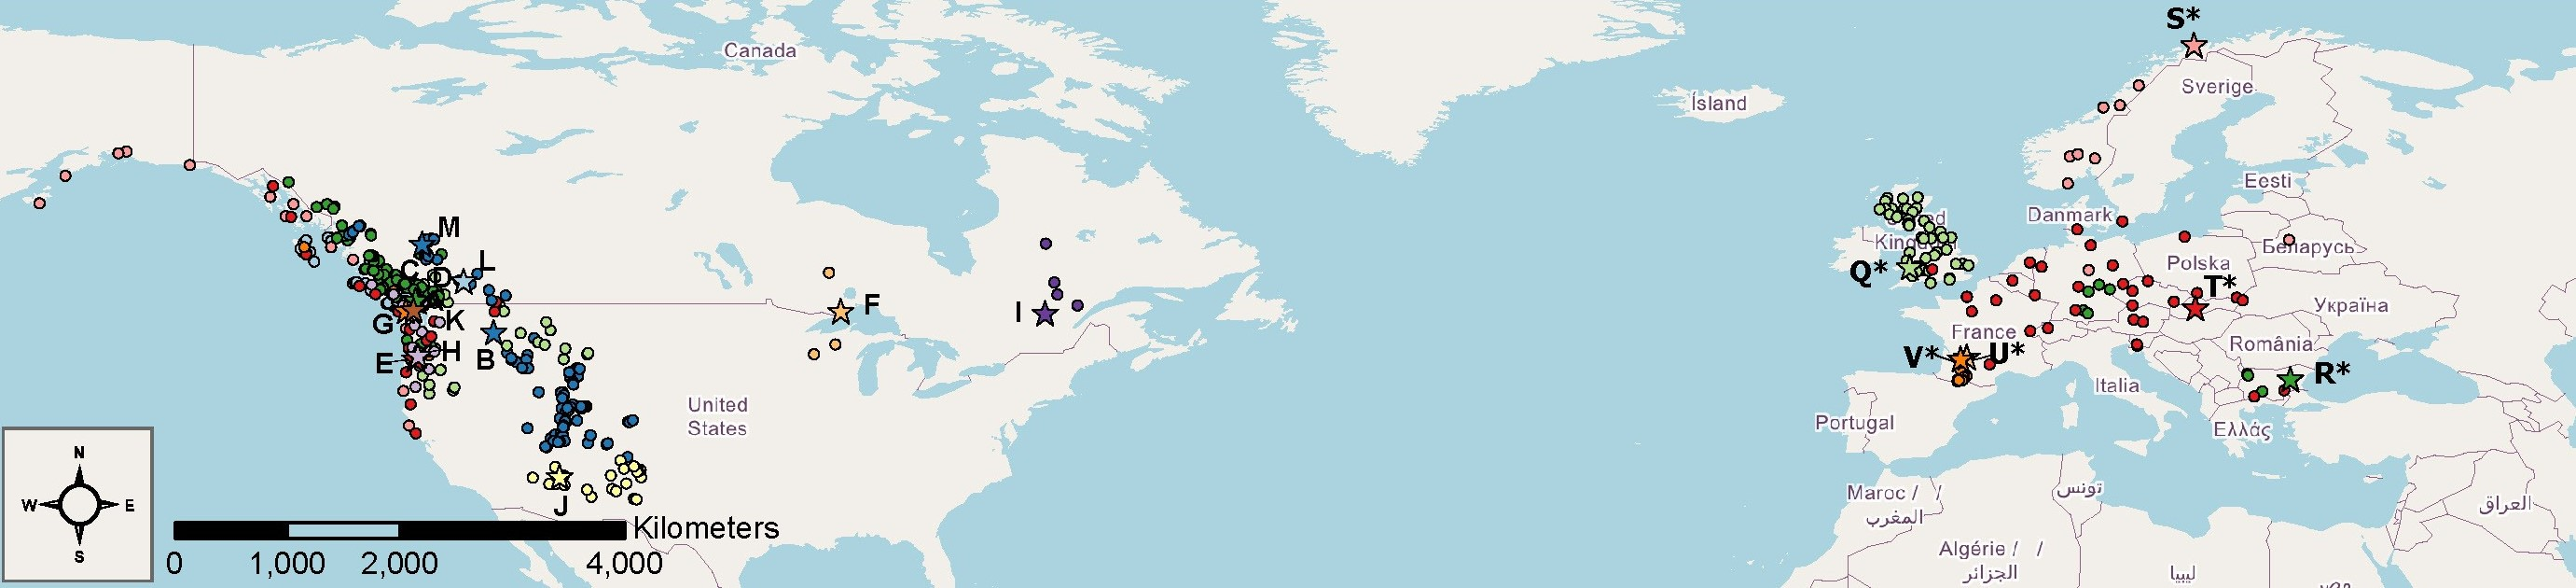
\includegraphics[width=\textwidth]{..//..//localadaptclim/Docs/figure_ms/map_gardens.jpg}
    \caption{Distribution of common gardens (denoted as stars) and provenances (denoted as circles) included in this meta-analysis. The distribution was skewed toward North America (12 North American studies versus 5 European studies). See Table.\ref{supplement-table:all_studies} in Supplements for information on selected studies.} 
    \label{figure:map_gardens}
\end{figure}
\newline
To understand how climatic differences, in addition to geographical differences, shape local adaptation in spring events we extracted several types of climate data using information about provenance latitude, longitude, and elevation from original publications. We estimated the mean annual temperature (MAT) for each provenance using the Climate Information Tool by Food and Agriculture Organization of the United Nations \citep{FAO2022}and ClimateWNA \citep{wang2016}. 

To examine more explicitly climate near spring events, we used gridded daily temperature data for 2011 to 2020 for all European and North American provenances and gardens from E-OBS and the `daymetr' package in R respectively \citep{cornes2018,hufkens2018}. Using these data we estimated how much the daily temperatures overlapped between garden and provenance locations, which we call `climate overlap.' For this we used the 'overlap' package in R to calculate the percentage overlap of the daily temperature of each provenance and their corresponding gardens in spring months (March to May) from 2011 to 2020. Finally, using the daily temperature data, we also calculated growing degree days (GDD), a commonly used heat accumulation measure to forecast phenological development in plants \citep{miller01}, for each provenance and garden, based on the accumulation of mean daily temperatures ($T_{m}$)from 2011 to 2020 above a baseline of 0$^{\circ}$C, from January 1 until budburst and leaf flush with the following formula: GDD = $\sum$($T_{m}$ - $0^{\circ}$C for $T_{m}$ $\ge$ $0^{\circ}$C; 0 for $T_{m}$ $\le$ $0^{\circ}$C). 

\subsection{Analyses}
To estimate clines in spring and fall phenological events across species we used Bayesian hierarchical models. We regressed DOY of events against geographical and climate predictors with partial pooling (sometimes called `random effects') on the intercept and slope for each species within each garden. Because most tree species were present in only one common garden in our dataset, it was impossible to fit garden and species separately, thus we treat each species within a garden as a unique group. Using posterior estimates for each species within a garden, we estimated effects of continent (North America vs. Europe) and species type (angiosperm vs. gymnosperm). All models were fit in `rstanarm' package (version 2.21.3; \citealp{brilleman2018}) using default priors, with 4 chains and 1000 sampling iterations per chain for a total of 4000 samples. We checked for model fit by ... [ADD here]. We present estimates as mean $\pm$ 90\% uncertainty intervals given parenthetically, unless otherwise stated. 

% alinaJuly20 I need help with ADD here (ping'd you in the old issue. I have removed all divergent transitions already)


% We pooled the timing of budburst and leaf flush into a single category of ‘spring events’ and the timing of bud set, leaf senescence, growth cessation, and leaf abscission into ‘fall events.’ Such pooling is justified because of the shared pressures from natural selection that govern these events \citep{Gill15}. 

\section{Results}
Our final dataset included seven angiosperm and eight gymnosperm species from 19 common gardens, encompassing 384 North American provenances and 101 European provenances, with observations from 1962 to 2019. Seven species also had fall event information available. 

Overall, spring events were not related to provenance latitude or MAT, neither across continents (latitude: 0.10 days/degree [-0.05 - 0.25]; MAT: -0.11 days/$^{\circ}$C [-0.34 - 0.12]) (Fig. \ref{figure:springfall_latmat}, Table. \ref{supplement-table:model_spring_lat} \& \ref{supplement-table:model_spring_mat} in Supplements), nor within North America (latitude: 0.10 days/degree [-0.06 - 0.26]; MAT: -0.09 days/$^{\circ}$C [-0.36 - 0.18]) or Europe (latitude: 0.10 days/degree [-0.23 - 0.42]; MAT:-0.16 days/$^{\circ}$C [-0.55 - 0.23]) (Fig.\ref{figure:continental_spptype_lat}A \& \ref{figure:continental_spptype_effect}A). Results were similar using other distance metrics in lieu of latitude (see Supplement Fig.\ref{supplement-figure:lat_distance} for results using the difference between provenance and garden latitude, and the spherical distance between provenance and garden).
% Spring events advanced slightly with provenance latitude in Europe spring events are slightly earlier where provenance MAT is lower (i.e., higher, more northern latitudes), though uncertainty intervals strongly overlapped zero. --- no longer the case

\begin{figure}[!h] 
    \centering
 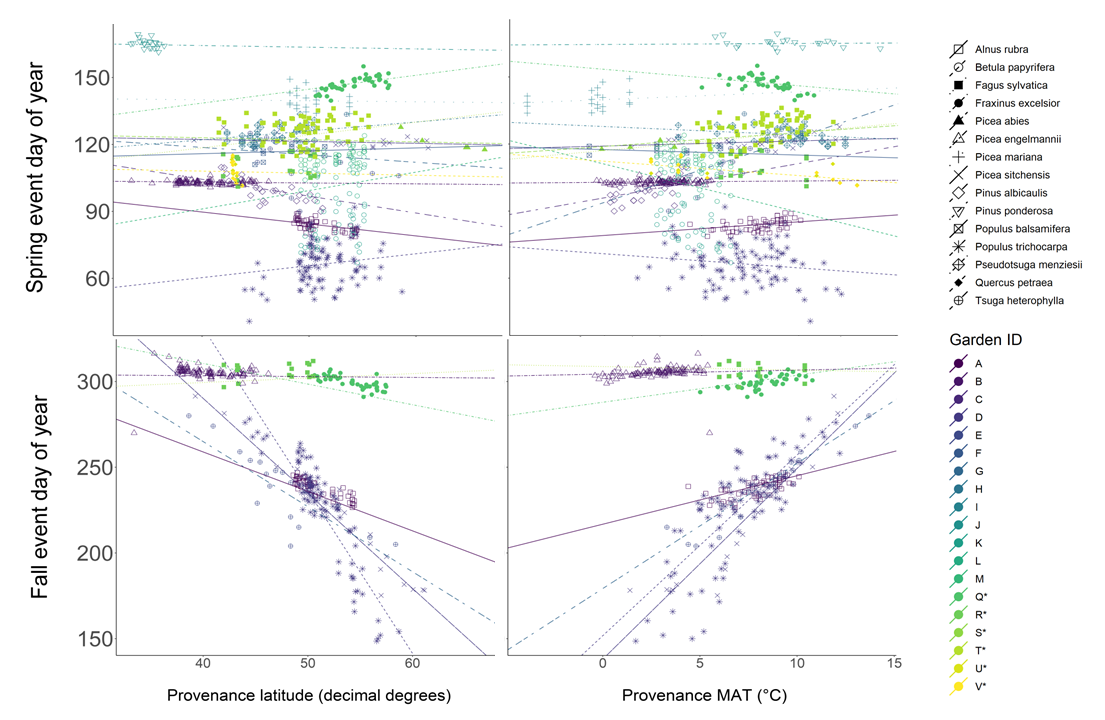
\includegraphics[width=\textwidth]{..//..//localadaptclim/Docs/figure_ms/springfall_latmat.jpg}
    \caption{Event day of year (DOY) in relation to provenance latitude and MAT, coded by symbol for species and color for garden with linear fits from hierarchical Bayesian models. Spring events shown on top and fall events at the bottom. European gardens and species are bolded and denoted by an asterisk (*). } 
    \label{figure:springfall_latmat}
\end{figure}


In contrast, fall events (e.g., budset, leaf senescence, leaf abscission) advanced strongly with provenance latitude (3.16 days/degree [2.87-3.45]) and the decrease in MAT (4.78 days/$^{\circ}$C [4.1 - 5.4]), meaning fall events were earlier where provenance MAT was lower (Fig. \ref{figure:springfall_latmat}, Table.\ref{supplement-table:model_fall_lat} \& \ref{supplement-table:model_fall_mat} in Supplements ). This relationship, however, was observed mostly in North America where fall events advanced 4.24 (3.95 - 4.53) days per degree northward, or 6.41 days (5.78 - 7.04) per degree decline in MAT ($^{\circ}$C), whereas in Europe such relationship was weaker: advance of 0.47 (0.21 - 1.17) days per degree northward, or 0.70 days (1.04 - 2.42) per degree decline in MAT ($^{\circ}$C) (Fig. \ref{figure:continental_spptype_effect}A).

% Note to us, see also https://github.com/lizzieinvancouver/localadaptclim/issues/25

Clines in fall phenology were stronger and more consistent whereas clines in spring phenology are weaker and somewhat varied in directionality. For fall events, only two field studies found no relationship (Fig. \ref{figure:springfall_latmat}): \emph{Fraxinus excelsior} from Garden Q* in the UK \citep{rosique22} and \emph{Fagus sylvatica} from Garden R* in Bulgaria \citep{petkova17}. Another study that found no relationship was the only greenhouse experiment included (\emph{Picea engelmannii} from Garden B in the USA, also included in \citealp{AitkenBemmels16}), which uniquely used the fall event of `the day by which seedling elongation had finished' \citep{rehfeldt94}. Spring event clines were always weak: all species x garden clines included 0 in their 90\% intervals.

\begin{figure}[!h] 
    \centering
 \includegraphics[width=\textwidth]{..//..//localadaptclim/Docs/figure_ms/continental_spptype_lat.jpg}
    \caption{Posterior distributions for the effect of provenance latitude across different continents and species types. Zero -- no effect -- is shown with a dashed line. Solid line and shading in posteriors represent mean and 50 percent interval. (A) Effect of latitude and continent on spring and fall event date (DOY). Fall events advanced strongly per degree northward, particularly notably in North America. (B) Effect of latitude and leaf type on spring and fall event date (DOY). As we move north, spring events slightly advanced in gymnosperms and delayed in angiosperms. Fall events advanced per degree northward for both species types.}
    \label{figure:continental_spptype_lat}
\end{figure}

\begin{figure}[!h] 
    \centering
 \includegraphics[width=\textwidth]{..//..//localadaptclim/Docs/figure_ms/continental_spptype_effect.jpg}
    \caption{Posterior distributions for the effect of MAT across different continents and species types. Zero -- no effect -- is shown with a dashed line. Solid line and shading in posteriors represent mean and 50 percent interval. (A) Effect of MAT and continent on spring and fall event date (DOY). Fall events advanced strongly with decreasing MAT, particularly notably in North America. (B) Effect of MAT and leaf type on spring and fall event date (DOY). As MAT increased, spring events slightly advanced in angiosperms and delayed in gymnosperms. Fall events delayed in warmer locations for both species types.}
    \label{figure:continental_spptype_effect}
\end{figure}

Effects of provenance latitude on fall events were similar across angiosperms and gymnosperms (Fig.\ref{figure:continental_spptype_lat}B). Spring events weakly diverged, delaying at a rate of 0.37 (0.15 - 0.59) days per degree north in angiosperms and advancing 0.23 (0.00 - 0.46) days per degree north in gymnosperms. Fall events advanced 3.18 (2.76 - 3.62) days per degree north in angiosperms and 3.14 (2.81-3.47) days per degree north in gymnosperms.
Effects of MAT on spring events also weakly diverged (Fig.\ref{figure:continental_spptype_effect}B). Spring events advanced 0.82 (0.54 - 1.11) days/$^{\circ}$C as MAT increased in angiosperms and delayed 0.76 (0.37 - 1.14) days/$^{\circ}$C as MAT increased in gymnosperms. Fall events delayed in warmer locations for both species types, but slightly more so for gymnosperms (6.23 days) than angiosperms (3.69 days) (Fig. \ref{figure:continental_spptype_effect}B).

While we expected that coarse metrics, such as latitude and MAT, would generally represent how similar the climates are between the provenances and gardens, we also estimated climate overlap in months much closer to the events to further test how much climate similarity between provenances and gardens predicts local adaptation. For spring events, we considered overlap across March to May. However, results were not qualitatively different than using MAT (See Fig. \ref{supplement-figure:overlap_scatterplot} in Supplements). We observed very weak effects of climate overlap on spring events (0.01 [0.02 - 0.03] days per one percent increase in climate overlap), nearly identical across angiosperms (0.02 [0.00 - 0.05]) and gymnosperms (0.04 [0.00 - 0.09]). Fall events advanced as climate overlap declined, but slightly more strongly for gymnosperms (advancing 0.72 [0.51 - 0.92] days per one percent decline in climate overlap) (Fig.\ref{supplement-figure:overlap_posterior} in Supplements).

% old graphs can be found in C:\Users\alina\Documents\git\localadaptclim\Output\plotMay15_two predictors_experiment
% refer to analyses\script_model_continent_spp_type_effect
% https://github.com/lizzieinvancouver/localadaptclim/issues/16

\section{Discussion}

Overall, our results demonstrated inconsistent and weak clines in spring events across North America and Europe. Specifically, there were weak diverging effects by species x garden groupings, which might be important and suggest different trends that mute an overall response. Fall events generally showed much stronger clines, suggesting a higher degree of local adaptation, especially in North America. While not directly testing plasticity or adaptation, our study suggests that spring events are highly plastic, and thus we predict that warming springs will continue to be tracked more closely phenologically by trees than warming fall temperatures. These interesting trends by species grouping for spring events and continent for fall events suggest that data on more species and greater information on important factors, such as their geographic location in relation to their origins and elevation, would aid forecasting. 
We found coarse metrics such as provenance latitude and MAT to be better predictors of timing than climate overlap and other metrics. Latitude and MAT appeared to well represent how similar the climates are between the provenances and gardens in months close to the events, at least in the narrow range of northern temperature and boreal forests we studied. 

\subsection{Variation across continents and species groupings}

Our results indicated that the effects of provenance latitude and MAT on fall events were similar across angiosperm and gymnosperm species: Fall events delay as MAT increases for both leaf types, slightly more so for gymnosperms, explained by sensitivity to day-length signals. However, the two leaf types exhibited slightly diverging trends in spring events:  advancing in angiosperms and delaying in most gymnosperms as MAT increases. Such differences make sense as timing of budburst and leafout varies by leaf type. Gymnosperms photosynthesize without leafout and thus generally leafout later than angiosperms, after much risk of spring frost \citep{panchen14}. Utilizing the early portion of the growing season can be especially critical for species in colder regions \citep{morin07, dantec15} and the ones with suboptimal shade tolerance \citep{richardson09}. 
Meanwhile, xylem anatomy also plays a part in determining spring timing due to the importance of vessel diameter to embolism risks induced by frost in spring. According to \citet{salk20}, species with narrow xylem such as coniferous gymnosperms and diffuse-porous angiosperms did not exhibit the consistent phenological trends shown in ring-porous species. Therefore, there might be additional differences if we have more species and more information on leafout timing and frost risk approach. 

\begin{enumerate}
\item Maybe also discuss ice sheet dynamics in Europe/North America, which could impact rates of adaptation.
\end{enumerate}
While we noticed more prominent clines in fall events in North America, there was no strong evidence of overall continental differences in spring events, which might again suggest a higher degree of plasticity in spring events. Meanwhile, most North American gardens and provenances included in this study were along the Pacific Northwest region \ref{}, which might mask the kind of climate pattern we were hoping to see from the entirety of North America.  % alinaJuly20: not sure about how to link to long-term climate history.

\subsection{Adaptation in spring vs fall phenology: Implications for climate change responses}
\begin{enumerate}
\item Our results suggest that current advances in spring phenology may continue, but delays in fall phenology could depend on speed of adaptation
\begin{enumerate}
\item Spring events appear highly plastic from these studies, which are good tests. 
\item Some previous chamber studies finding potential adaptation (cited in Ettinger et al. 2020 Nature Climate Change, I believe -- check the paper and supp) but these could be influenced by chilling at the provenance site, whereas gardens do not have this effect
\item Previous work has suggested strong clines in fall phenology and our findings back this up... 
\item These findings have important implications for growing discussion of how shifting phenology and tree growth relate as our results suggest there are strong limits on shifts in fall phenology (Zohner2023 and other papers such as Zani 2020 -- need a couple sentences here) % D. Zani, T. W. Crowther, L. Mo, S. S. Renner, C. M. Zohner, Increased growing-season productivity drives earlier autumn leaf senescence in temperate trees. Science 370, 1066–1071 (2020).
\end{enumerate}
\item These trends likely vary by species and depend on frost tolerance strategy
\begin{enumerate}
\item If current advances in spring phenology continues it could mean shifts in spring frost etc., but differences across species suggest this will not impact all species the same. 
\item In temperate and boreal environments, the optimal timing for spring growth initiation is determined by a balance of avoiding late spring frost and having a long growing season \citep{alberto11, lenz16, allevato19} ... further Plants that budburst earlier can take advantage of a longer growing season and avoid competition  \citep{guo22}....  and species vary in how the balance this tradeoff. 
\end{enumerate}
\item Species may also vary in whether we predict co- or counter-gradient relationships with spring phenology
\begin{enumerate}
\item Fall events were always co-gradient
\item Spring events were more varied -- some appeared to be co or counter ... 
\item Add some discussion of what this might mean (one idea is that spring leafout sets up flowering and thus some counter-gradient could aid gene flow over larger areas? Other ideas you have?) and cite some of the relevant papers. 
\end{enumerate}
\item All of this critical to predicting not just phenological change, but range expansions with climate change: An accurate understanding of how environmental conditions might influence species distribution at a continental scale is critical for future range shift prediction.
\begin{enumerate}
\item Implications of small differences in spring phenology could mean different gene flow etc. 
\item the degree of adaptation dictated by climate change also differs across different geographical areas \citep{Loarie09}. 
\item Mention elevational results here? 
\end{enumerate}
\end{enumerate}

% \item Implications of our results on animals: Many terrestrial animals time their breeding season to coincide with the availability of food resources. For example, migratory birds arrive at breeding grounds amidst the peaking of insects \citep{hallfors20}. Many butterfly species ensure their larvae have an ample food supply by synchronizing their egg-laying with the phenology of their host plants \citep{rytteri21,posle18}. Similarly, the migration and spawning of many marine organisms are closely tied to water temperature and the availability of planktonic food sources \citep{genner10}. Such synchronization enables them to provide optimal food for their young during critical growth stages. Therefore, climate warming and the associated changes in spring phenology timing, such as earlier leafout or insect emergence due to climate change, can disrupt this synchronization and negatively impact animal populations \citep{wann19,renner18, chu17}. 




 %REFS
 % savolainenAREES -- have not read recently but sounds relevant
 % gauzere2020 -- cite and read
 % \cite{chang2021} and \cite{chuine2016} -- relevant for discussion of chilling
 % See also Salk 2020 paper


\section{Figures}



\bibliography{bibliography_local_adaptation.bib}



\section{Acknowledgement}
We thank S. Aitken,  I. Chuine, R. Guy, C Korner and Y. Vitasse for reviewing our list of papers for possible additional common garden studies. 


\end{document}




% helping with abstract language
% Alberto16
% "On the basis of the patterns of quantitative variation for 19 adaptation-related traits studied in 59 tree species (mostly temperate and boreal species from the Northern hemisphere), we found that genetic differentiation between populations and clinal variation along environmental gradients were very common (respectively, 90% and 78% of cases)."

% formatting code resources
% https://github.com/lizzieinvancouver/ospree/blob/master/docs/ranges/ranges_outline.tex
% https://github.com/lizzieinvancouver/ospree/blob/master/docs/traits/Traitors_Manuscript_supp.Rnw

